
% !TEX encoding = UTF-8 Unicode
\documentclass[a4paper]{article}

\setcounter{tocdepth}{1}

\usepackage{color}
\usepackage{url}
\usepackage[T2A]{fontenc} % enable Cyrillic fonts
\usepackage[utf8]{inputenc} % make weird characters work
\usepackage{graphicx}
\usepackage{subcaption}

\usepackage[english,serbianc]{babel}

\usepackage[unicode]{hyperref}
\hypersetup{colorlinks,citecolor=green,filecolor=green,linkcolor=blue,urlcolor=blue}

\usepackage{listings}

\definecolor{mygreen}{rgb}{0,0.6,0}
\definecolor{mygray}{rgb}{0.5,0.5,0.5}
\definecolor{mymauve}{rgb}{0.58,0,0.82}

\lstset{ 
  backgroundcolor=\color{white},
  basicstyle=\scriptsize\ttfamily,  
  breakatwhitespace=false,         
  breaklines=true,                 
  captionpos=b,                   
  commentstyle=\color{mygreen},   
  deletekeywords={...},           
  escapeinside={\%*}{*)},          
  extendedchars=true,              
  firstnumber=1000,                
  frame=single,	                   
  keepspaces=true,                 
  keywordstyle=\color{blue},       
  language=Python,                 
  morekeywords={*,...},            
  numbers=left,                    
  numbersep=5pt,                   
  numberstyle=\tiny\color{mygray},
  rulecolor=\color{black},        
  showspaces=false,               
  showstringspaces=false,          
  showtabs=false,                  
  stepnumber=2,                   
  stringstyle=\color{mymauve},     
  tabsize=2,	                   
  title=\lstname                   
}

\begin{document}

\title{\Large Решавање проблема максималног ахроматског броја\\ \small{Научни рад у оквиру курса Рачунарска интелигенција\\ Универзитет у Београду, Математички факултет}}

\author{Душан Пантелић\\ pantelic.dusan@protonmail.com}

\maketitle

\begin{center}
	
\includegraphics[width=3cm]{images/pmf.png}
\end{center}

\abstract{
Кроз овај рад читалац ће бити упућен у проблем максималног ахроматског броја, као и у решавање истог. Пре свега, шта представља максимални ахроматски број, његов значај, примену, али и проблеме при његовом одређивању. Представљени су алгоритми за решавање проблема и њихова компарација, као и њихове позитивне и негативне стране. Читалац ће такође добити увид у експерименталне податке извршавања представљених алгоритама са примењеним статистичким методама зарад стварања шире слике о практичној примени. На крају рада сумирани су закључци истраживања и изложени правци за даље истраживање и унапређивање.
\tableofcontents

\newpage

\section{Увод}
\label{sec:intro}
Познавање општих концепата теорије графова је неопходно за разумевање рада, тако да се пропоручује претходно упознавање са материјом помоћу релевантне литературе \footnote{Пример литературе \cite{graphteoryintro}.}.
	\subsection{Бојење графа и ахроматски број}
	Правилно бојење графа представља додељивање боја чворовима графа, тако да никоја два суседна чвора немају исту боју. Граф можемо бојити на више начине, стога бојење графа не мора бити јединствено, већ може садржати различити број боја, где избор боја није релевантан.
	Бојење графа са n боја називамо n-бојење, а уколико важи да за сваки пар различитих боја постоје два суседна чвора графа којима су те боје додељене, то бојење називамо комплетно n-бојење.\\
	Хроматски број графа G, у ознаци \(\chi(G)\), представља минималан број n тако да постоји комплетно n-бојење тог графа. Ахроматски број графа G, у ознаци \(\psi(G)\), представља максималан број n тако да постоји комплетно n-бојење тог графа.
	
	\subsection{Особине ахроматског броја}
	Нека је n број чворова неког графа G, тада можемо уочити да важи следеће: 1 $\le$ \(\chi(G)\) $\le$ \(\psi(G)\) $\le$ n. Ахроматски број такође можемо представити као максимални број партиција у свим партиционисањима низа чворова, при чему унутар партиције не сме бити суседних чворова и за сваки пар партиција мора постојати барем једна грана која повезује те две партиције. Горе наведена дефиниција је погоднија за касније имплементирање алгоритамских решења. Јанакакис и Гаврил су доказали да је проблем налажења ахроматског броја НП-комплетан \cite{yanandgav}.
	
	\subsection{Значај налажења ахроматског броја}
	Решавање проблема ахроматског и хроматског броја су специјални случајеви проблема бојења графа, где уз правилно бојење захтевамо да број боја буде максималан односно минималан. Једно правилно бојење графа може бити решење судоку слагалице, разних проблема планирања, као и проблема алокације регистра \cite{coloringapplications}. Кроз пример планирања летова авиона где сваки чвор представља лет, а грана између два чвора представља да се летови преклапају, видимо да правилно бојење овако представљеног графа распоређује авионе групи летова мећу којима нема преклапања летова. Приметимо такође да тражењем ахроматског броја у претходном примеру заправо тражимо максималан број авиона да покрију све групе летова где између група летова мора бити преклапања(ради мањег чекања) чиме добијамо растерећење авио саобраћаја, док тражењем хроматског броја тражимо најмањи број авиона који покривају летове.  



\section{Решење проблема}
\label{sec:problem-solution}

\subsection{Алгоритам провере исправности бојења}
Овај алгоритам не решава проблем ахроматског броја, али се користи у свим осталим алгоритмима који ће бити обрађени, тако да ћемо га одвојити као целину и приказати његов псеудо-код. \\

\begin{lstlisting}[caption={Псеудо-код провере исправности бојења},frame=single]
function proveri_bojenje(bojenje):
	for (svaka boja u bojenju):
		if (boja sadrzi susedne cvorove):
			return False
	
	for (svaki par boja u bojenju):
		if (ne postoji grana izmedju parova boja ):
			return False
			
	return True
\end{lstlisting}
 
\subsection{Алгоритам исцрпне претраге}
Најпоузданији али и временски најзахтевнији начин решава проблема ахроматског броја је алгоритам исцрпне претраге. Идеја алгоритма је да се за сваки могући број боја генришу сва могућа бојења, при чему тражимо највећи број боја за који постоји валидно бојење. \\ 

\begin{lstlisting}[caption={Псеудо-код алгоритма исцрпне претраге},frame=single]
function nadji_ahromatski_broj(graf):
	ahromatski_broj = -1
	for (svaki moguci broj boja grafa br):
		for (bojenje grafa u svim mogucim bojenjima sa br boja):
			if (proveri_bojenje(bojenje)):
				ahromatski_broj = br
				break
		
return ahromatski_broj 
\end{lstlisting}

\textbf{Предности алгоритма:} Решење је оптимално.

\textbf{Мане алгоритма:} Експоненцијална сложеност.

\subsection{Генетски алгоритам}
Решење проблема генетским алгоритмом је направљено модификацијом алгоритма приказаном у \cite{geneticachr}. У наставку је приказан псеудокод, као и описи свих битнијих карактеристика алгоритма. \\

\begin{lstlisting}[caption={Псеудо-код генетског алгоритма},frame=single]
function genetski_algoritam():
	populacija = random_bojenja_grafa()
	while (nije ispunjen maksimalan broj iteracija i nije dostignuto optimalno resenje):
		sort(populacija)
		zadrzi_cetvrtinu_najboljih_jedinki()
		for (ostatak jedinki):
			selktuj_roditelje()
			ukrsti_roditelje()
			izvrsi_mutaciju()
	return populacija
\end{lstlisting}

\textbf{Критеријум заустављања:} Алгоритам се зауставља када је достигнут максималан број итерација, или у случају када је познато оптимално решење зауставља се када нека од јединки садржи оптимално решење.

\textbf{Сортирање популације:} Популацију сортирамо на основу прилагођености јединке коју добијамо функцијом прилагођености опадајуће. 

\textbf{Функција прилагођености:} Функцију прилагођености рачунамо као количник броја боја коришћеног при бојењу и броја грешака које доводе до неисправног бојења. Уколико је број грешака једнак нули јединку награђујемо тако што множимо број боја са константом већом од један. Треба бити обазрив прилоком избора награде за валидно бојење. Премала награда доводи до тога да валидна решења испадну из популације, док превелика награда фаворизује валидна решења и не дозвољава да се развију можда оптималнија решења чиме популација конвергира ка локалном оптимуму.

\textbf{Елитизам:} Задржавамо четвртину најбољих јединки како би обезбедили да наставе живот непромењене.

\textbf{Селекција:} Бирамо насумично две јединке, при чему свака јединка има исту шансу да буде изабрана.

\textbf{Укрштање:} Низ чворова графа делимо на три дела насумичне величине. Прво дете узима за први део чворова боје првог родитеља, за други боје другог родитеља и за трећи опет боје првог родитеља. За друго дете важи обратно.

\textbf{Мутација:} Свака јединка са задатом вероватноћом мења боју насумичног чвора у такоће насумичну боју.

\textbf{Предности алгоритма:} Извршава се у разумном временском периоду.

\textbf{Мане алгоритма:} Решење није увек оптимално, а некада решење није валидно бојење.

\textbf{Могућа унапређења:} Уколико након завршетка алгоритма популација не садржи валидно решења један од начина превазилажења овог проблема је коришћење алгоритма мудрости роја честица описаног у \cite{wisdom}. Овај алгоритам није имплементиран, али идеја је да се најбоља половина решења локално претражује до проналаска валидног решења тако што ће чворови најбољег решења који нарушавају валидност променити боју у најзаступљенију боју за тај чвор у осталим јединкама.

\subsection{Хибридни генетски алгоритам}
Претходно описан алгоритам можемо надоградити тако што ћемо приликом сваке итерације најбољу и најгору јединку обрадити алгоритмом симулираног каљења. Симулирано каљење, иако се некада користило као самосталан алгоритам за проблем бојења графа, не даје довољно добра решења у пракси \cite{annealing}. Без обзира на горе наведено, конвергенцију популације можемо убрзати хибридизацијом генетског алгоритма тј. додавањем симулираног каљења.\\

\begin{lstlisting}[caption={Псеудо-код симулираног каљења},frame=single]
function simulirano_kaljenje():
	while (nije dostignut maksimalan broj iteracija za kaljenje):
		if (validno_bojenje):
			podeli cvorove nasumicne boje na dva dela i drugom delu dodaj novu boju
		else:
			zameni boje na dva nasumicno izabrana cvora
		
		if (promena donosi bolju prilagodjenost):
			prihvati_promenu
		else if (kontrolni_parametar > nasumicnog_broja):
			prihvati_promenu()
		else:
			odbaci_promenu()
		azuriraj_kontrolni_parametar()
\end{lstlisting}

\textbf{Напомена:} Контролну променљиву ажурирати тако да како итерације одмичу тако је и мања вероватноћа прихватања неповољне промене. Не треба ни одмах бити сувише мала да не би остали у локалном оптимуму.

\textbf{Предности алгоритма:} Може убрзати конвергенцију популације ка оптималном решењу, али и извадити популацију из локалног оптимума.

\textbf{Мане алгоритма:} Могуће је изгубити оптимално решење прихватањем неповољније промене.

\section{Експериментални резултати}
\label{sec:experimet-results}
У наставку ће бити приказани експериментални резултати, њихова визуелизација као и поређење резултата. За тест примере коришћени су насумично генерисани графови са бројем чворова између 2 и 14. Графови су сачувани у gml формату и можете их пронаћи на \url{https://github.com/pantelic-dusan/maximum-achromatic-number/random_graphs}. Tестови су извршавани на платформи \url{https://cgc.sbgenomics.com} на инстанци x1.32xlarge(3840 SSD, 128vCPUs, 1952GB RAM), и сви тест резултати су доступни на \url{https://github.com/pantelic-dusan/maximum-achromatic-number/test_results} у JSON формату.

\subsection{Визуализација података}
Део резултата, који поред броја чворова и грана за сваки од горе наведених алгоритама приказује и редом резултат њиховог извршавања као и време протекло током извршавања, приказан је на \ref{data_view}.

\begin{figure}[h!]
	\centering
	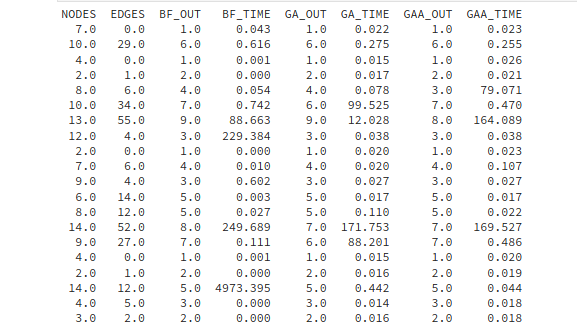
\includegraphics[width=10cm, height=5cm]{images/data_view.png}
	\caption{Пример резултата}
	\label{data_view}
\end{figure}

Такође приказивањем података о врему извршавања алгоритама редом на \ref{times}, можемо видети напредак друга два алгоритма у односу на алгоритам исцрпне претраге.
\begin{figure}[h!]
	\centering
	\begin{subfigure}{.3\textwidth}
		\centering
		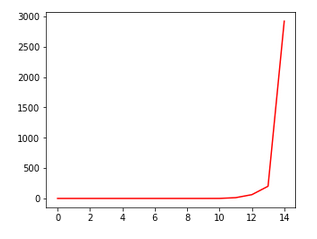
\includegraphics[width=\linewidth]{images/bf_time.png}
	\end{subfigure}
	%
	\begin{subfigure}{.3\textwidth}
		\centering
		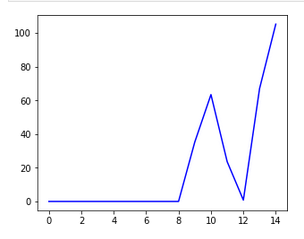
\includegraphics[width=\linewidth]{images/ga_time.png}
	\end{subfigure}
	%
	\begin{subfigure}{.3\textwidth}
		\centering
		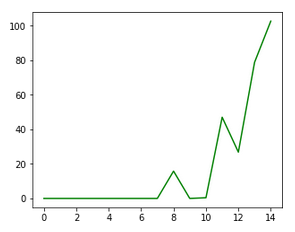
\includegraphics[width=\linewidth]{images/gaa_time.png}
	\end{subfigure}
\caption{Просечно време извршавања у односу на број чворова}
\label{times}
\end{figure}

\subsection{Поређење генетског алгоритма са и без симулираног каљења}
Поређењем редом просечног времена извршавања и просечног броја итерација гентских алгоритама са и без симулираног каљења на тест резултатима, долазимо до закључка да додавањем симулираног каљења незнатно побољшавамо перформансе генетског алгоритма, што можемо видети на слици \ref{performance_comp}.

\begin{figure}[h!]
	\centering
	\begin{subfigure}{.4\textwidth}
		\centering
		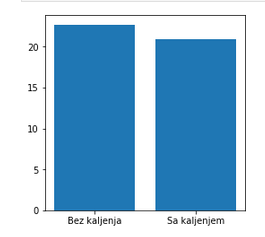
\includegraphics[width=\linewidth]{images/time_compare.png}
	\end{subfigure}
	%
	\begin{subfigure}{.4\textwidth}
		\centering
		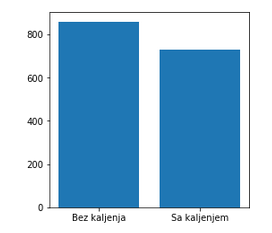
\includegraphics[width=\linewidth]{images/iters_compare.png}
	\end{subfigure}
	\caption{Поређење перформанси генетског алготитма са и без каљења}
	\label{performance_comp}
\end{figure}

Такође поређењем, као на слици \ref{optimal_comp}, редом процента исправних решења и процента оптималних решења, долазимо до закључка да генетски алгоритам са каљењем благо побољшава вероватноћу добијања оптималног решења и да оба алгоритма дају исправна решења.

\begin{figure}[h!]
	\centering
	\begin{subfigure}{.4\textwidth}
		\centering
		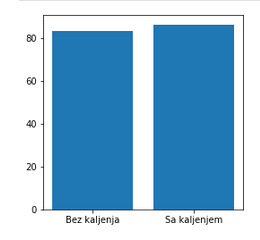
\includegraphics[width=\linewidth]{images/optimals_compare.png}
	\end{subfigure}
	%
	\begin{subfigure}{.4\textwidth}
		\centering
		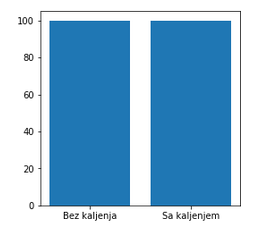
\includegraphics[width=\linewidth]{images/valids_compare.png}
	\end{subfigure}
	\caption{Поређење оптималности генетског алготитма са и без каљења}
	\label{optimal_comp}
\end{figure}

\section{Закључак}
\label{sec:conclusion}
Собзиром на значај обрађене теме потребно је стално унапређивати постојеће методе за решавање овог проблема. Обрађена су три алгоритма, која са свим својим предностима и манама, нису довољно добра за проблеме који захтевају изузетну прецизност и брзину решавања. Побољшања су могућа тако што ћемо на основу статистичких резултата кориговати константе алгоритма као што су број итерација, величина популације, фактор мутације, израчунавање прилагођености, или у случају опције са симулираним каљењем тражимо најповољнији број итерација и фактор опадања контролне променљиве.\\

Читаоцу се препоручује да настави самостално унапрећивање обраћених алгоритама, али и покушај комбиновања са другим методама. Такође је препорука да се изуче и друге врсте алгоритама попут
Дејвид-Путманове методе описане у \cite{annealing}, оптимизација колонијом мрава описане у \cite{aop}, али и других доступних решења.

sdsdfsdfsdfsd dsdsdfdsfs
\addcontentsline{toc}{section}{Литература}
\appendix
\bibliography{maximum-achromatic-number} 
\bibliographystyle{plain}

\newpage
\end{document}